\section{Closure}
\label{sec:closure}

Define a strategy for closure. (LDD+MW+SC+JCM)

\subsection{Introduction}

We have seen that the new \nfit code gives us access to very powerful and
modern fitting tools. With great power comes great responsibility, we have already
seen examples of some kind of overfitting with the new code - producing PDFs
with wiggly behaviour and incredibly good fits to the data. This affect is
well demonstrated in the \nfit paper and can be seen in Figure \ref{fig:v3pdf}

\begin{figure}[!h]
    \centering
    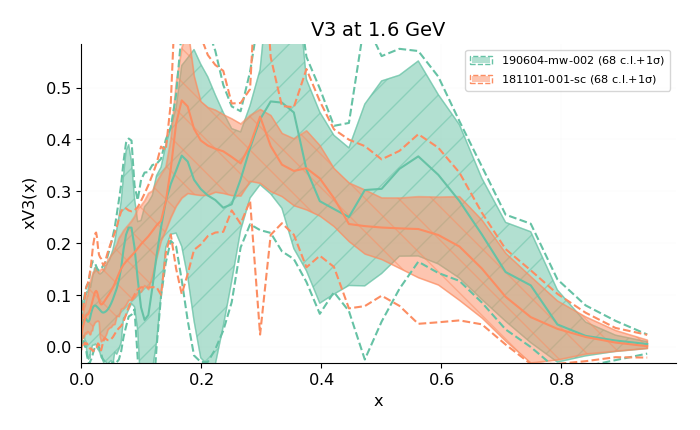
\includegraphics[width=0.8\textwidth]{plot_pdfs_V3.png}
    \caption{
        Figure showing wiggly behaviour of v3 PDF when using the new fitting code.
        }
    \label{fig:v3pdf}
\end{figure}

This leaves us with a few questions: Can we discriminate against this
architecture/minimiser choice in a closure test using the closure estimators?
Is this just flat directions in the DIS only fit? Is there a good prescription
for combatting this effect.

There has already been a study purely on the data which shows that by having a test
set which is used in the hyper parameter scan which seperates out completely a dataset
or series of datasets the hyper optimiser lands on a notably smaller network which reduces
the amount of redundant features in the PDF. Do we need to consider the same kind of test
set in the closure tests so that the closure test estimators can be calculated both in and
out of sample - where in sample refers to the dataset appearing in either the training
or validation set which is used for stopping.

\subsection{results}

\subsubsection*{Closure on pseudodata from large architecture PDF}

As a sanity check we can run a closure test with the higher parameterisation
which gave wiggly PDFs in a fit to pseudo data which is generated from the
wiggly PDF. This is to see if the features we see in the space of the PDF are
somehow picked up by the data in such a way that we can refit the same underlying
function.

This is a brute force way of trying to understand whether the features in the PDF
are just flat directions in the loss or are some kind of feature of the data. To
test this I am taking as input a wiggly PDF, and then just generating the MC
replica (level 2) noise on top of this, and so there is no level 1 fluctuation.
The test is to see if the functional form of the replicas matches the input PDF.

The full report comparing the closure fit to underlying can be found here:
\href{https://vp.nnpdf.science/tHdjyBVTQEOlfkNjUXPMFQ==}{\bf{report}}

The closure tests estimators are not particularly useful here, largely because
there is no level 1 noise. The main feature is the PDF plots are much smoother
for the closure in nearly all instances, which suggests that the extra features
in the underlying PDF are not translated into the space of data by the
\texttt{FastKernel} tables.

From this test we are would be persuaded that the underlying PDF was just fitting
flat directions in the loss and that the fluctuations in the PDF shouldn't be
taken too seriously.

\subsubsection*{Closures with different level 1 shift}

A second sanity check was to run two different closures changing nothing but the
seed used to generate the level 1 shifts on the pseudodata. This was a test I
wanted to run to check how important it was that we considered two closures ran
not only on the same datasets but also with the same level 1 noise. In other
words, how robust are the statistical estimators on the level 1 noise? In particular
we added bootstrap sampling to some of the statistical estimators and it would
be good to know if the errorbar given by a bootstrap represents the distribution
under different level 1 shifts.

The full report can be found here:
\href{https://vp.nnpdf.science/mbcTUd6-TQmQFvaGd37bkg==}{\bf{report}}. In particular
one will note that the variance is unchanged within statistics as you would expect
but the bias and the $\dcs$ both appear to depend heavily on the level 1 noise.

This serves as a warning that the closure tests should be ran with the same level
1 data if they are to be compared.


\subsubsection*{Closures on \texttt{MSTW2008nlo68cl}}

Now we take the smooth \texttt{MSTW2008nlo68cl} as input. We fit this
with both the conservative architecture, roughly corresponding to the number of
parameters used in NNPDF3.1, and the larger architecture found by the hyperopt
routine. The objective here is to see if we can use the closure test estimators
to distinguish and discriminate between the two fits.

All reports can be found on Wiki

Report to underlying for conservative architecture:
\href{https://vp.nnpdf.science/9qr4qCK2RHePHehBpgxBdQ==/}{\bf{report}}

larger architecture:
\href{https://vp.nnpdf.science/pdm9Y1fjTw21nhlzjzErjw==/}{\bf{report}}

Comparison report:
\href{https://vp.nnpdf.science/lQjtB-lnRy263IhAYCTw1Q==/}{\bf{report}}

we see that the delta chi2 is comparable for both fits, however the bias is
is generally lower for the conservative architecture, as well as the variance.
It seems that there is a wider spread of replicas for the larger architecture,
but this hasn't improved the fit of the central replica on the underlying law.
From the value of $\dcs$ we would say, however, that the fit hasn't moved away
from the underlying law towards the level 1 data, and appears to have just
produced a worse quality fit. The lower variance is expected for the smaller
architecture, but the interesting thing is that there hasn't been a gain in
the bias.
